\begin{frame}
    \frametitle{Kanonische Transformationen sind Gruppe}
    
    Zwei kanonische Transformationen:
    \begin{align*}
        \sum_{i=1}^{n} (p_i \delta q_i - P_i \delta Q_i) &= \delta S \\
        \sum_{i=1}^{n} (P_i \delta Q_i - \bar{p}_i \delta \bar{q}_i) &= \delta \bar{S}
    \end{align*}
    
    Summe ist wieder kanonische Transformation:
        \begin{align*}
        \sum_{i=1}^{n} (p_i \delta q_i - \bar{p}_i \delta \bar{q}_i) &= \delta (S + \bar{S}) 
        \end{align*}
        
    Für jedes $S=S(q_1,\ldots,q_n; Q_1,\ldots,Q_n;t),\quad t>0$ gibt es eine Transformation.
    
\end{frame}


\begin{frame}
    \begin{align*}
        t,&\qquad t+\Delta t \\
        Q_k &= q_k + \Delta q_k \\
        P_k &= p_k + \Delta p_k
    \end{align*}
    
    \begin{align*}
        \Longrightarrow \qquad \Delta q_i &= \frac{\partial B}{\partial p_i} \Delta t,\\
                         \Delta p_i &= -\frac{\partial B}{\partial q_i} \Delta t
    \end{align*}
    
    mit
    
    \begin{displaymath}
        B(q_1,\ldots,q_n; p_1,\ldots,p_n;t) = -\frac{\partial S}{\partial t}
    \end{displaymath}
\end{frame}

\begin{frame}
\hspace*{-2.2cm}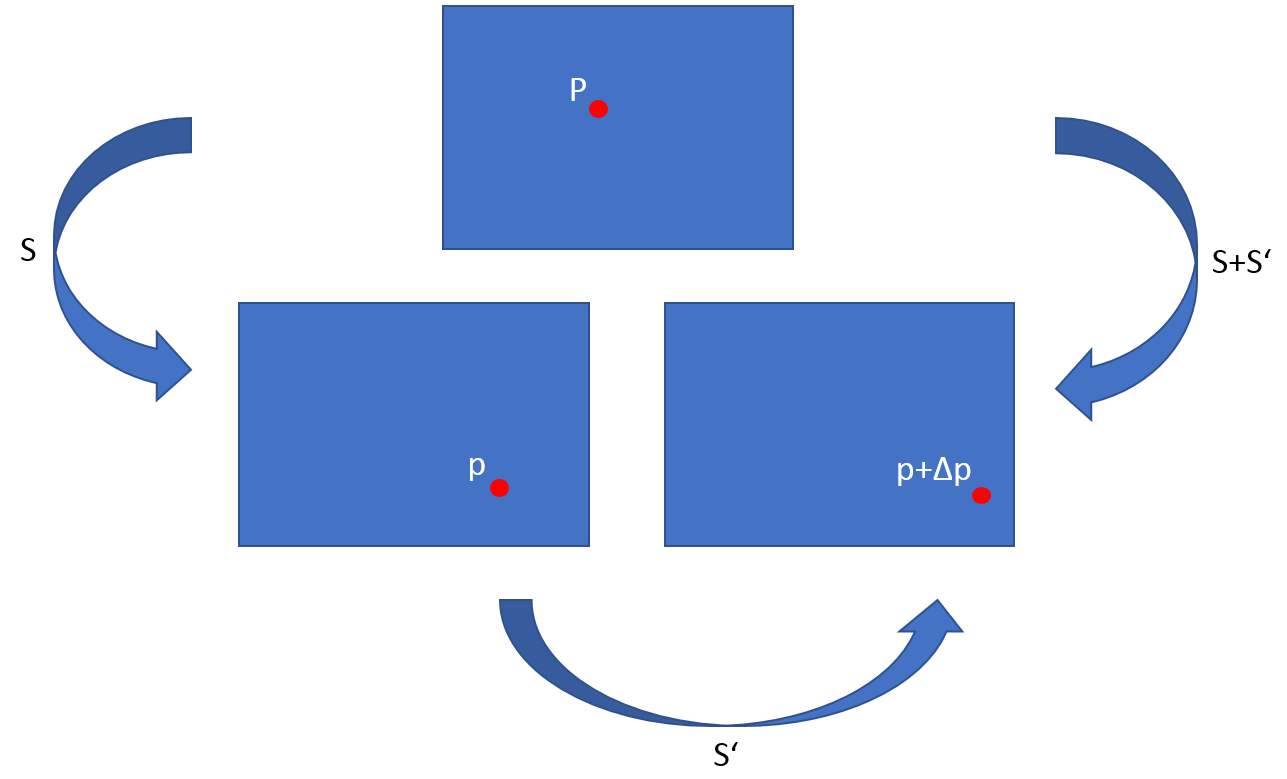
\includegraphics[scale=0.375]{images/ImagTrans}
\end{frame}

\begin{frame}
    \hspace*{-2.2cm}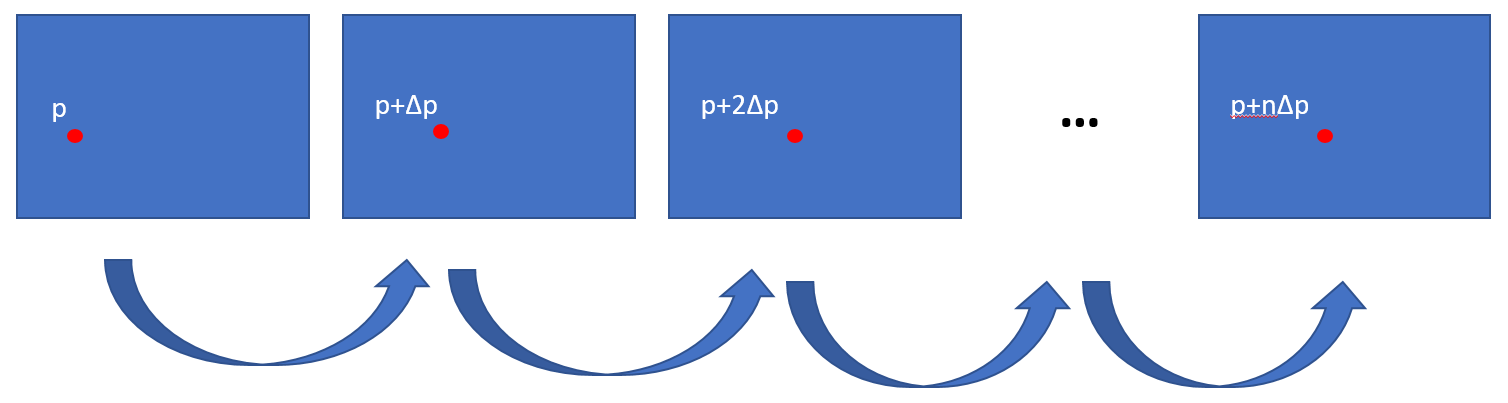
\includegraphics[scale=0.322]{images/TransFlow}
\end{frame}

\begin{frame}
    \begin{align*}
    \Delta q_i &= \frac{\partial B}{\partial p_i} \Delta t,\\
    \Delta p_i &= -\frac{\partial B}{\partial q_i} \Delta t \\[5mm]
      \Delta t &\longrightarrow 0 \\[5mm]
    \frac{dq_i}{dt}  &= \frac{\partial B}{\partial p_i},\\
    \frac{dp_i}{dt} &= -\frac{\partial B}{\partial q_i} 
    \end{align*}
    
    \begin{center} $\rightarrow$ Das sind die kanonischen Bewegungsgleichungen, wobei $B=H$. \end{center}

\end{frame}